% STOCKBACK whitepaper. Build: cd whitepaper && tectonic stockback-whitepaper.tex && mv stockback-whitepaper.pdf STOCKBACK-Whitepaper.pdf
\documentclass[10.5pt,letterpaper]{article}

\usepackage[margin=1in,headheight=14pt]{geometry}
\usepackage{amsmath,amsthm}
\usepackage{newpxtext,newpxmath}
\setmonofont{Inconsolatazi4-Regular.otf}[BoldFont=Inconsolatazi4-Bold.otf,Scale=0.86]
\usepackage{microtype}
\usepackage{mathtools}
\usepackage{booktabs,tabularx,array,multirow}
\usepackage{xcolor,graphicx}
\usepackage{tikz}
\usetikzlibrary{arrows.meta,positioning,fit,backgrounds,calc,shapes.geometric}
\usepackage{pgfplots}
\pgfplotsset{compat=1.18}
\usepgfplotslibrary{fillbetween}
\usepackage{enumitem}
\usepackage{caption}
\usepackage{fancyhdr}
\usepackage{titlesec}
\usepackage{float}
\usepackage[hidelinks]{hyperref}
\usepackage{fontawesome5}
\newcommand{\inr}{{\scalebox{0.82}{\faRupeeSign}}\kern0.04em}

% ---------------------------------------------------------------- brand
\definecolor{shu}{HTML}{C83A2F}
\definecolor{shudeep}{HTML}{8F211D}
\definecolor{sumi}{HTML}{171717}
\definecolor{washi}{HTML}{F4EFE3}
\definecolor{washideep}{HTML}{EBE3D2}
\definecolor{stone}{HTML}{8A8378}
\definecolor{ai}{HTML}{2F6F9F}
\hypersetup{colorlinks=true,linkcolor=shudeep,citecolor=shudeep,urlcolor=shudeep}

\titleformat{\section}{\large\bfseries\color{sumi}}{\textcolor{shu}{\thesection}}{0.8em}{}
\titleformat{\subsection}{\normalsize\bfseries\color{sumi}}{\textcolor{shu}{\thesubsection}}{0.7em}{}
\titlespacing*{\section}{0pt}{1.6ex plus .4ex}{0.9ex}
\titlespacing*{\subsection}{0pt}{1.2ex plus .3ex}{0.6ex}

\captionsetup{font=small,labelfont={bf,color=shudeep},margin=0.5em}
\setlist{itemsep=2pt,topsep=4pt}
\setlength{\parskip}{3pt}

\pagestyle{fancy}
\fancyhf{}
\fancyhead[L]{\small\color{stone}STOCKBACK \textperiodcentered{} Signed purchase evidence, admin-less ownership}
\fancyhead[R]{\small\color{stone}\thepage}
\renewcommand{\headrulewidth}{0.3pt}
\renewcommand{\headrule}{\hbox to\headwidth{\color{washideep}\leaders\hrule height \headrulewidth\hfill}}

\newtheorem{proposition}{Proposition}
\newtheorem{lemma}{Lemma}
\theoremstyle{definition}
\newtheorem{definition}{Definition}
\theoremstyle{remark}
\newtheorem*{remark}{Remark}

\newcommand{\Ok}{\textsc{Ok}}
\newcommand{\ttt}[1]{\texttt{#1}}
\newcommand{\cat}{\mathbin{\|}}
\newcommand{\kk}{\operatorname{keccak256}}
\newcommand{\enc}{\operatorname{abi.encode}}
\DeclareMathOperator{\Accept}{Accept}
\DeclareMathOperator{\Verify}{Verify}

% the hanko seal
\newcommand{\seal}[1]{%
  \tikz[baseline=-0.6ex]{\fill[shu] (0,0) circle (#1);
  \node[text=washi,font=\bfseries\fontsize{#1*1.5cm}{#1*1.5cm}\selectfont] at (0,0) {S};}}

\begin{document}

% ================================================================ title
\thispagestyle{empty}
\begin{tikzpicture}[remember picture,overlay]
  \fill[washi] (current page.north west) rectangle ([yshift=-3.05in]current page.north east);
  \fill[shu] ([xshift=-1.15in,yshift=-0.95in]current page.north east) circle (0.42in);
  \node[text=washi,font=\bfseries\fontsize{40}{40}\selectfont] at ([xshift=-1.15in,yshift=-0.95in]current page.north east) {S};
\end{tikzpicture}

\vspace*{-0.35in}
\noindent{\color{shudeep}\small\bfseries WHITEPAPER \textperiodcentered{} v1.0 \textperiodcentered{} OCTOBER 2026}\par\vspace{10pt}
\noindent\begin{minipage}{5.2in}\raggedright{\fontsize{24}{28}\selectfont\bfseries\color{sumi}STOCKBACK: Signed Purchase Evidence and Admin-less Ownership Settlement on Arbitrum Stylus\par}\end{minipage}\par
\vspace{10pt}
\noindent{\large\color{sumi}Every receipt, sealed. \textcolor{stone}{Scan. Prove. Own.}\par}
\vspace{10pt}
\noindent{\small Project STOCKBACK \textperiodcentered{} Arbitrum Open House Singapore Buildathon 2026\\
Live: \ttt{stockbacks.vercel.app} \textperiodcentered{} Robinhood Chain testnet (chain 46630)\\
Source: \ttt{github.com/notwen123/STOCKBACK}\par}
\vspace{22pt}

\begin{center}
\begin{minipage}{0.9\textwidth}
\small
\noindent{\bfseries\color{sumi}Abstract.}
Reward programs that pay on a purchase must first believe the purchase happened, and almost all of them
believe a receipt photograph. That belief no longer holds: in a 2026 paired study, people picked an
AI-edited receipt from its authentic counterpart at chance (0.501), and the best forensic detectors reached
an AUC of 0.53--0.60~\cite{wu2026forger}. We present \emph{STOCKBACK}, a protocol that moves the trust origin of a
purchase from pixels to a signature and settles each verified purchase as shares of a brand-specific,
admin-less ERC-4626 vault. A merchant point-of-sale signs every reward-relevant field of a receipt with
Ed25519; an attester accepts the receipt only if that signature verifies, the receipt has not expired, the
brand is supported and the receipt has never been claimed, then signs a hashes-only EIP-712 claim bound to
the claimant's wallet. On-chain, a single transaction checks the attestation in Rust on Arbitrum Stylus,
burns a per-receipt nullifier, applies eligibility, reward caps and a sponsor budget, and deposits into the
vault on the user's behalf. We formalize the claim calculus, prove replay resistance and a closed-form bound
on the loss from an attester-key compromise, and report measurements on Robinhood Chain testnet. Verifying
Ed25519 in Stylus costs $65{,}088$ gas per signature against $608{,}542$ for the best available Solidity
implementation (both linear fits, $R^2>0.9999$), up to $9.2\times$ cheaper, and fits $100$ signatures in one
transaction where Solidity cannot fit $53$. The reference deployment has settled 13 real claims and funded a
reward budget in USDG through a live swap; it is covered
by 83 Foundry tests including fuzzing and invariants, 5 Rust tests, 42 receipt-signing and live-integration
tests and an 11-step browser suite. We state plainly what is simulated (the merchant), what is mocked (every
brand asset) and what is not yet built.
\end{minipage}
\end{center}

\vspace{6pt}
\noindent{\small\textbf{Keywords:} proof of purchase; receipt forgery; Ed25519; Arbitrum Stylus; EIP-712; nullifiers; ERC-4626; loyalty programs; Robinhood Chain.}

% ================================================================ 1
\section{Introduction}

A purchase leaves evidence behind: a receipt, a UPI or PayNow reference, an order email. Every system that rewards
purchases, refunds damaged goods or reimburses expenses converts that evidence into money, and nearly all of
them accept the evidence in its weakest form, an image. Generative image models have changed the cost of that
choice. Changing one number on a receipt photograph now takes ``under a second for a few cents''; when shown an
authentic receipt and its AI-edited twin side by side, 120 human inspectors chose correctly
50.1\% of the time; forensic detectors that score 0.85--0.96 AUC on traditional tampering fall to
0.585--0.599 on the same documents edited by a modern model~\cite{wu2026forger}. Refund-fraud evidence shows the same
pattern: multimodal models catch only 23\% of AI-fabricated damage photos while specialized detectors
falsely accuse honest customers~\cite{yan2026fraudbench}. The economics are well understood: when fabrication becomes cheap
before verification becomes worthwhile, high-trust markets that delay checking attract fraud first~\cite{yin2026trust}.
A new reward program that trusts photographs is exactly such a market.

\paragraph{Scope: a global protocol, launched rail-first.} Nothing in the protocol is tied to one country. Each brand's
currency is an ISO-4217 code stored on-chain, geography is delegated to a jurisdiction-policy adapter, and sponsors fund
budgets in USDG, a dollar stablecoin. Launching a brand in SGD or USD is one configuration call, not a redeployment. We
target first the markets where purchases already leave a digital merchant trail: Singapore (PayNow and SGQR) and India,
where UPI processed 24.07 billion payments in September 2026 alone~\cite{npci2026}. The reference deployment is priced in
INR for that reason.

The reward side is also weak. Consumers belong to 14.8 loyalty programs on average and use 6.7; 73\% find
them too complicated; roughly 60\% of coalition programs fail within ten years, and operators can expire or
devalue balances at will~\cite{oamen2025rewards}. Points are a liability on someone else's balance sheet, not property.

STOCKBACK addresses both halves. On the evidence side, trust moves from the image to a signature produced at the
point of sale, and every claim carries an explicit \emph{evidence tier} that states what was and was not
established. On the settlement side, a verified purchase becomes shares of an ERC-4626 vault with no owner, no
pause and no sweep: once minted, only the holder can move them.

\begin{figure}[t]
\centering
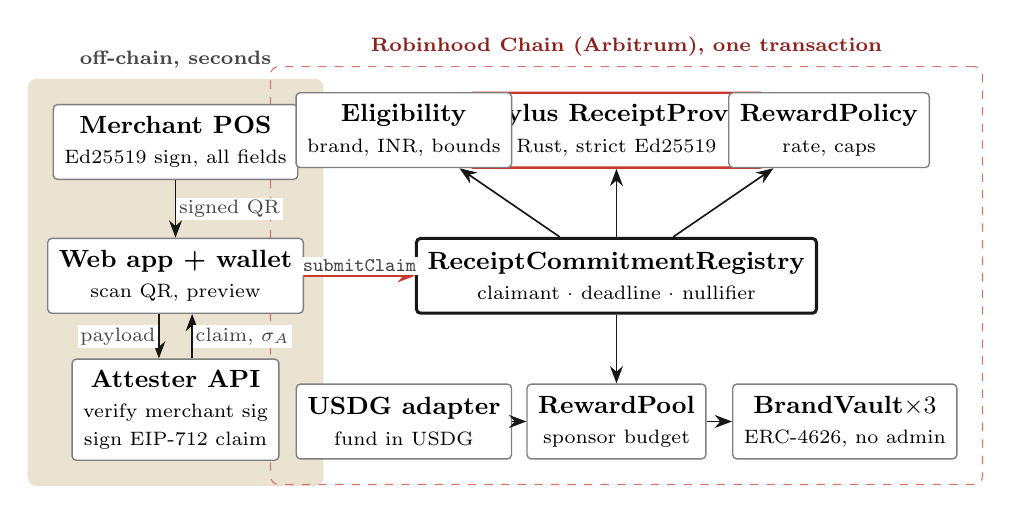
\begin{tikzpicture}[
  font=\small,
  box/.style={draw=sumi!55,fill=white,rounded corners=1.5pt,align=center,minimum height=0.95cm,inner sep=4pt,line width=0.5pt},
  key/.style={box,draw=shu,line width=0.9pt},
  arr/.style={-{Stealth[length=2.2mm]},line width=0.6pt,color=sumi},
  red/.style={-{Stealth[length=2.2mm]},line width=0.9pt,color=shu},
  lab/.style={font=\scriptsize,color=sumi!80,fill=white,inner sep=1pt}]
  % off-chain
  \node[box] (pos) at (0,2.6) {\textbf{Merchant POS}\\ \scriptsize Ed25519 sign, all fields};
  \node[box] (app) at (0,0.9) {\textbf{Web app + wallet}\\ \scriptsize scan QR, preview};
  \node[box] (att) at (0,-0.8) {\textbf{Attester API}\\ \scriptsize verify merchant sig\\[-1pt]\scriptsize sign EIP-712 claim};
  \draw[arr] (pos) -- node[lab,right] {signed QR} (app);
  \draw[arr] ([xshift=-6pt]app.south) -- node[lab,left] {payload} ([xshift=-6pt]att.north);
  \draw[arr] ([xshift=6pt]att.north) -- node[lab,right] {claim, $\sigma_A$} ([xshift=6pt]app.south);
  % on-chain
  \node[box,line width=1.1pt,draw=sumi] (reg) at (5.6,0.9) {\textbf{ReceiptCommitmentRegistry}\\ \scriptsize claimant \textperiodcentered{} deadline \textperiodcentered{} nullifier};
  \node[key] (sty) at (5.6,2.75) {\textbf{Stylus ReceiptProver}\\ \scriptsize Rust, strict Ed25519};
  \node[box] (eli) at (2.9,2.75) {\textbf{Eligibility}\\ \scriptsize brand, INR, bounds};
  \node[box] (rp) at (8.3,2.75) {\textbf{RewardPolicy}\\ \scriptsize rate, caps};
  \node[box] (pool) at (5.6,-0.95) {\textbf{RewardPool}\\ \scriptsize sponsor budget};
  \node[box] (vault) at (8.5,-0.95) {\textbf{BrandVault}$\times3$\\ \scriptsize ERC-4626, no admin};
  \node[box] (usdg) at (2.9,-0.95) {\textbf{USDG adapter}\\ \scriptsize fund in USDG};
  \draw[red] (app) -- node[lab,above] {\ttt{submitClaim}} (reg);
  \draw[arr] (reg) -- (sty); \draw[arr] (reg) -- (eli); \draw[arr] (reg) -- (rp);
  \draw[arr] (reg) -- (pool); \draw[arr] (pool) -- (vault); \draw[arr] (usdg) -- (pool);
  \begin{scope}[on background layer]
    \node[fill=washideep,rounded corners=3pt,fit=(pos)(att),inner sep=9pt,label={[font=\scriptsize\bfseries,color=sumi!80]north:off-chain, seconds}] {};
    \node[draw=shu!70,dashed,rounded corners=3pt,fit=(eli)(rp)(usdg)(vault)(sty),inner sep=9pt,label={[font=\scriptsize\bfseries,color=shudeep]north:Robinhood Chain (Arbitrum), one transaction}] {};
  \end{scope}
\end{tikzpicture}
\caption{STOCKBACK architecture. The registry is the only contract that consumes caps or spends budget; the verifier
only answers yes or no; vaults have no administrator. Everything inside the dashed box runs in the single
\ttt{submitClaim} transaction.}
\label{fig:arch}
\end{figure}

\subsection{Contributions}
\begin{itemize}
  \item A \textbf{claim calculus} (Section~\ref{sec:calculus}): an EIP-712 purchase claim whose identifiers are hashed off-chain,
        a nullifier independent of claimant, amount and deadline, and an acceptance predicate evaluated in one
        transaction, with a proof of replay resistance and a closed-form bound on attester-compromise loss.
  \item \textbf{Merchant-signed receipts} (Section~\ref{sec:merchant}): a versioned canonical message over eight fields, field grammars
        that make line injection impossible, and an attester that verifies the merchant signature against a public
        key it holds, never the private key.
  \item \textbf{Ed25519 on Arbitrum Stylus} (Section~\ref{sec:stylus}): a Rust verifier behind the same ABI as the Solidity verifier,
        with a measured linear gas model and the resulting batch ceilings under the 32M per-transaction cap.
  \item \textbf{Sponsor funding in USDG} (Section~\ref{sec:arch}): budgets are topped up in USDG through an adapter that swaps
        into the brand asset with oracle-bounded slippage, exercised by a live funding transaction (Section~\ref{sec:eval}).
  \item An \textbf{evaluation against the live chain} (Section~\ref{sec:eval}) and \textbf{findings} that only building and testing
        against deployed code surfaced (Section~\ref{sec:findings}), including one defect in the upstream code this project forked.
\end{itemize}

% ================================================================ 2
\section{Threat Model and Design Goals}\label{sec:threat}

We consider six principals. The \emph{shopper} holds a wallet and is untrusted. The \emph{merchant point-of-sale (POS)}
holds an Ed25519 signing key and is trusted to sign only sales that happened; in this deployment it is simulated.
The \emph{attester} holds the merchant public key and its own Ed25519 key, and is trusted for the checks it performs,
not beyond them. The \emph{registry and verifier} are contracts, trusted for integrity of their code. The
\emph{sponsor} funds a per-brand budget and is trusted only with its own funds. The \emph{owner} configures policies and
caps and is the single administrative key (Section~\ref{sec:limits}).

\paragraph{Goals.}
\textbf{(G1) Field binding:} no reward-relevant field (brand, amount, currency, receipt, merchant, time) can change
between the point of sale and the chain without invalidating a signature.
\textbf{(G2) Once per receipt:} a receipt yields at most one reward, for anyone, regardless of claimant, amount or deadline.
\textbf{(G3) Bounded authority:} every key, including the attester's and the owner's, can lose at most a capped,
pre-funded amount; no key can touch shares already minted.
\textbf{(G4) No personal data on-chain:} only hashes, an amount, a currency and timestamps.
\textbf{(G5) Honest evidence:} every claim states its evidence tier; a photograph is never presented as proof of purchase.
\textbf{(G6) Fail closed:} a missing key or an unverifiable receipt stops the claim; nothing is signed on a guess.

\paragraph{Non-goals.} Proof of personhood (one human, one wallet); protection against a compromised merchant key;
recovering rewards for refunded purchases (no hold period yet); and confidentiality of the purchase amount.

% ================================================================ 3
\section{System Architecture}\label{sec:arch}



Figure~\ref{fig:arch} shows the deployed system: eight Solidity contracts (OpenZeppelin~5, solc 0.8.24, 791 lines),
one Rust contract on Stylus (251 lines), and a Next.js web application with the attester and simulated POS as
server routes. Contracts are single-purpose and acyclic; none is upgradeable. Table~\ref{tab:authority} gives the
authority analysis: which component can produce which effect.

\begin{table}[!htb]
\centering\small
\caption{Authority analysis. Each row is a component, each column an effect. The last column is empty by
construction: no code path lets any key move shares a user already holds.}
\label{tab:authority}
\begin{tabular}{@{}lccccc@{}}
\toprule
Component & Sign claim & Burn nullifier & Spend budget & Change rules & Move user shares\\
\midrule
Merchant POS key   & receipt only & --- & --- & --- & ---\\
Attester key       & yes & --- & --- & --- & ---\\
Stylus verifier    & --- & --- & --- & --- & ---\\
Registry (code)    & --- & yes & via pool & --- & ---\\
RewardPool (code)  & --- & --- & yes\textsuperscript{a} & --- & ---\\
Owner key          & --- & --- & unallocated only & yes & ---\\
Shopper wallet     & --- & --- & --- & --- & \textbf{own only}\\
\bottomrule
\end{tabular}\\[3pt]
\footnotesize\textsuperscript{a}Only when called by the registry; \ttt{allocate} reverts for any other caller.
\end{table}

\subsection{Evidence tiers}
The on-chain path is identical for every claim. What differs is what the attester checked before signing, and
STOCKBACK labels it on every screen (Table~\ref{tab:tiers}).

\begin{table}[H]
\centering\small
\caption{Evidence tiers.}
\label{tab:tiers}
\begin{tabularx}{\textwidth}{@{}c>{\raggedright}p{3.3cm}>{\raggedright}Xc@{}}
\toprule
Tier & Evidence & What it establishes & Status\\
\midrule
1 & Merchant-signed receipt (QR) & Every field unaltered since the merchant key signed it. Merchant simulated in this deployment. & Live demo\\
2 & Attested photo / OCR & Only that the attester signed what it was given; authenticity is not established. & Live demo\\
3 & Payment or order proof (zkTLS) & Provenance from the payment or order source itself~\cite{zhang2020deco}. & Roadmap\\
\bottomrule
\end{tabularx}
\end{table}

% ================================================================ 4
\section{The Claim Calculus}\label{sec:calculus}

\subsection{Claims and commitments}
A purchase claim is the tuple
\begin{equation}
c = (w,\; b,\; m,\; r,\; a,\; \kappa,\; t_p,\; t_d),
\end{equation}
where $w$ is the claimant's address, $b$ the brand identifier, $m=\kk(\text{merchant})$, $a$ the amount in minor units
(paise), $\kappa$ an ISO-4217 code, $t_p$ the purchase time and $t_d$ the attestation deadline. The receipt reference
$\rho$ never appears; the claim carries a salted hash
\begin{equation}\label{eq:receipt}
r = \kk\!\big(\enc(\kk(s),\, \rho)\big),
\end{equation}
where $s$ is a secret attester salt, so short references such as an eight-digit invoice number cannot be
brute-forced from public data. The claim's commitment and the digest the attester signs are
\begin{align}
H(c) &= \kk\!\big(\enc(\tau_c, w, b, m, r, a, \kappa, t_p, t_d)\big),\\
\mathrm{DS} &= \kk\!\big(\enc(\tau_D, \texttt{"STOCKBACK"}, \texttt{"1"}, \chi, \mathcal R)\big),\\
d(c) &= \kk\!\big(\texttt{0x1901} \cat \mathrm{DS} \cat H(c)\big),\label{eq:digest}
\end{align}
with $\tau_c,\tau_D$ the EIP-712 type hashes~\cite{eip712}, $\chi$ the chain identifier and $\mathcal R$ the registry address.
Binding $\chi$ and $\mathcal R$ into the domain makes a signature useless on any other chain or deployment.

\subsection{Nullifiers}
\begin{definition}[Nullifier]
For a claim $c$,
\[ \nu(c) = \kk\!\big(\enc(\kk(\texttt{"STOCKBACK\_NULLIFIER\_V1"}),\, m,\, r)\big). \]
\end{definition}

The nullifier depends only on the merchant and the salted receipt hash. It deliberately excludes the claimant,
amount, brand and deadline, so none of them can be varied to re-use a receipt.

\begin{proposition}[Once per receipt]\label{prop:replay}
Let $N$ be the registry's set of burned nullifiers. For any two accepted claims $c\neq c'$ with the same merchant and
receipt reference, at most one is accepted. More strongly, $\nu(c)=\nu(c')$ for every pair of claims that agree on $(m,r)$,
regardless of $(w,b,a,\kappa,t_p,t_d)$.
\end{proposition}
\begin{proof}
$\nu$ is a function of $(m,r)$ alone. Acceptance requires $\nu(c)\notin N$ and inserts $\nu(c)$ into $N$ before any
external call (checks-effects-interactions), within one transaction under a reentrancy guard. The second claim
therefore observes $\nu(c')=\nu(c)\in N$ and is rejected with \textsc{NullifierUsed}. Collisions of distinct $(m,r)$
pairs require a keccak256 collision. The property is exercised by unit tests, a 1{,}000-run fuzz test over claimant, amount and deadline, and the
invariant \ttt{invariant\_noReplay}.
\end{proof}

\subsection{Acceptance}
Let $\Verify_V(d,\sigma)$ be the active verifier (Ed25519 in Stylus or ECDSA in Solidity) with attester allowlist $V$.
A claim with attestation $\sigma$ submitted by sender $u$ at block time $t$ is accepted iff
\begin{equation}\label{eq:accept}
\Accept(c,\sigma) \iff
\underbrace{u=w}_{\text{binding}} \wedge
\underbrace{t\le t_d}_{\text{fresh}} \wedge
\underbrace{\nu(c)\notin N}_{\text{once}} \wedge
\underbrace{\Verify_V(d(c),\sigma)}_{\text{attested}} \wedge
\underbrace{E_b(c)}_{\text{eligible}} \wedge
\underbrace{Q_b(c)}_{\text{within caps}} \wedge
\underbrace{R(c)\le B_b}_{\text{funded}},
\end{equation}
evaluated in exactly that order, the first failing conjunct naming one of sixteen status codes. Eligibility is
\begin{equation}
E_b(c) \iff \mathrm{active}_b \wedge \kappa=\kappa_b \wedge a_b^{\min}\le a\le a_b^{\max} \wedge t_p\le t \wedge t-t_p\le T_{\mathrm{age}},
\end{equation}
with live values $a^{\min}=$~\inr 100, $a^{\max}=$~\inr 5{,}00{,}000 and $T_{\mathrm{age}}=30$ days. Because the order is fixed and
every check before the transfer is a pure function of state, \ttt{previewClaim} returns exactly the status that
\ttt{submitClaim} would revert with, which the interface uses to explain a rejection before the wallet opens.

\subsection{Rewards and caps}
For brand $b$ with rate $\rho_b$ (asset base units per minor currency unit, $10^{18}$-scaled) and multiplier
$\mu_b\in(0,3]$ (in basis points),
\begin{equation}\label{eq:reward}
R(c) = \min\!\left( \left\lfloor \frac{a\,\rho_b\,\mu_b}{10^{18}\cdot 10^{4}} \right\rfloor,\; C_b^{\mathrm{claim}} \right).
\end{equation}
The product is computed with a 512-bit intermediate (\ttt{Math.mulDiv}), so it cannot overflow for any
$a<2^{128}$. Daily caps \emph{reject} rather than clip:
\begin{equation}\label{eq:caps}
Q_b(c) \iff U_b(w,\delta)+R(c)\le C_b^{\mathrm{user}} \;\wedge\; D_b(\delta)+R(c)\le C_b^{\mathrm{brand}},\qquad \delta=\lfloor t/86400\rfloor .
\end{equation}
Rejecting matters: a clipped claim would burn the nullifier for a partial reward, while a rejected claim leaves the
receipt claimable on a later day. Table~\ref{tab:params} lists the live parameters.

\begin{table}[!htb]
\centering\small
\caption{Live reward parameters on Robinhood Chain testnet, read from \ttt{RewardPolicy} and \ttt{RewardPool} on 2 October 2026. Units are demo asset units ($10^{18}$ base units).}
\label{tab:params}
\begin{tabular}{@{}lccccc@{}}
\toprule
Brand & Effective rate & $C^{\mathrm{claim}}$ & $C^{\mathrm{user}}$ per day & $C^{\mathrm{brand}}$ per day & Budget $B_b$\\
\midrule
NIKE & 0.75\% of value & 100 & 300 & 100{,}000 & $\approx 1.01\times10^6$\\
AAPL & 0.50\% of value & 100 & 300 & 100{,}000 & $\approx 1.00\times10^6$\\
SBUX & 1.00\% of value & 100 & 300 & 100{,}000 & $\approx 1.00\times10^6$\\
\bottomrule
\end{tabular}
\end{table}

For example, a \inr 2{,}000 Nike purchase has $a=200{,}000$ paise and $\rho=7.5\times10^{13}$, giving $R=15$ units, the value
observed in every Nike claim on chain.

\subsection{Settlement into an admin-less vault}
The pool deposits $R(c)$ of the brand asset into the brand's ERC-4626 vault~\cite{erc4626} with receiver $w$. With total
assets $A$ and share supply $S$, OpenZeppelin's virtual-share accounting with decimals offset $\delta_v=6$ mints
\begin{equation}
\mathrm{shares}(R) = \left\lfloor R\cdot\frac{S+10^{\delta_v}}{A+1}\right\rfloor .
\end{equation}
The offset makes a first-depositor inflation attack unprofitable, which a dedicated vault test checks.
The vault has no owner, pause or sweep. Pausing the registry stops new claims but never redemptions.

\subsection{Bounded loss under key compromise}
\begin{proposition}[Attester-compromise bound]\label{prop:bound}
Suppose an adversary obtains the attester key at time $t_0$ and the owner pauses the registry at $t_0+\Delta$. Then the
total value the adversary can extract from brand $b$ is at most
\begin{equation}\label{eq:bound}
L_b \;\le\; \min\!\Big( B_b,\; \big\lceil \Delta/86400 \big\rceil \cdot C_b^{\mathrm{brand}} \Big),
\end{equation}
and shares minted before $t_0$ are unaffected.
\end{proposition}
\begin{proof}
Every acceptance passes through the registry, which consumes $D_b(\delta)$ and $B_b$ (Eqs.~\ref{eq:caps},~\ref{eq:accept}).
The per-user cap gives no protection, since fresh wallets are free, so the binding limits are the per-brand daily cap
over the days touched and the funded budget. No component holds authority over minted shares (Table~\ref{tab:authority}).
\end{proof}
With live parameters, a compromise left unanswered for a full day costs at most 100{,}000 demo units per brand, and
draining a budget takes about ten days. The response requires no redeploy: pause, replace the key in the Stylus verifier's
attester allowlist (\ttt{set\_attester}), unpause. The same bound covers abuse of the public demo POS.

% ================================================================ 5
\section{Merchant-Signed Receipts}\label{sec:merchant}

\subsection{Canonical message}
A merchant receipt is the field vector
\[ \mathbf{f} = (\text{merchantId},\ \text{merchantName},\ \text{brand},\ \text{receiptId},\ \text{amount},\ \text{currency},\ t_{\mathrm{iss}},\ t_{\mathrm{exp}}). \]
Each field $f_i$ must match a fixed grammar $\Gamma_i$. For example, the amount is a positive integer of at most
14 digits in minor units, and the receipt identifier is 8 to 64 characters from \ttt{[A-Za-z0-9-]}. Validity also
requires $t_{\mathrm{exp}}>t_{\mathrm{iss}}$ and a validity window of at most 30 days.
The signed bytes are
\begin{equation}\label{eq:canon}
M(\mathbf f) = \texttt{"STOCKBACK-MERCHANT-RECEIPT-V1"} \;\Vert\; \big\Vert_{i=1}^{8}\; \big(\texttt{"\textbackslash n"} \cat k_i \cat \texttt{"="} \cat f_i\big),
\end{equation}
and the receipt travels as $\texttt{SBR1}.\mathrm{b64url}(\mathbf f).\mathrm{b64url}(\sigma_M)$ with $\sigma_M=\mathrm{Sign}_{sk_M}(M(\mathbf f))$.

\begin{lemma}[No field injection]
No $\Gamma_i$ admits a newline or \texttt{=}, so $M$ is injective on valid field vectors: two distinct valid vectors
never produce the same message.
\end{lemma}
\begin{proof}
Every field is preceded by a newline and a fixed key in a fixed order, and no field value can contain either
delimiter. The message therefore parses uniquely back into $\mathbf f$.
\end{proof}

By the lemma and the unforgeability of Ed25519~\cite{rfc8032}, changing any field, including the amount, brand, receipt
identifier or either timestamp, invalidates $\sigma_M$, which is goal G1.

\subsection{Verification and attestation}
The attester holds only the merchant public key $pk_M$. Given a payload it computes
\begin{equation}\label{eq:mverify}
\mathrm{ok}(\mathbf f,\sigma_M) \iff \mathrm{Ed25519.Verify}_{pk_M}(M(\mathbf f),\sigma_M) \wedge \text{issuedAt}\le t+120 \wedge t<\text{expiresAt} \wedge \text{brand}\in\mathcal B,
\end{equation}
checking the signature \emph{first} so the more specific errors cannot be used to probe unsigned edits. It then derives
every reward-relevant claim field from $\mathbf f$, namespacing the receipt reference by merchant
($\rho = \text{merchantId}\,\Vert\,\texttt{:}\,\Vert\,\text{receiptId}$) so two merchants cannot collide on one nullifier, and
clamping the claim deadline to the receipt's expiry, $t_d=\min(t+3600,\ \text{expiresAt})$. Before returning the
attestation it dry-runs Eq.~\ref{eq:accept} and refuses a receipt whose nullifier is already burned. Table~\ref{tab:reject}
lists every rejection and the test that exercises it.

\begin{table}[!htb]
\centering\small
\caption{Merchant receipt rejections. Each is covered by a unit test (20 in total) and, where marked, by the live
integration suite against the deployed contracts.}
\label{tab:reject}
\begin{tabular}{@{}llcl@{}}
\toprule
Input & Outcome & HTTP & Live test\\
\midrule
Any of 8 fields altered after signing & \texttt{bad\_signature} & 401 & amount, brand, receiptId, issuedAt\\
Random 64-byte signature & \texttt{bad\_signature} & 401 & yes\\
Signed by an untrusted key & \texttt{bad\_signature} & 401 & yes\\
Expired receipt & \texttt{expired} & 410 & yes\\
Validly signed, unsupported brand & \texttt{unsupported\_brand} & 422 & yes\\
Malformed or non-string payload & \texttt{malformed} & 400 & yes\\
Receipt already claimed (any wallet) & \texttt{already\_claimed} & 409 & yes, after a real claim\\
Merchant or attester key missing & fail closed & 503 & yes\\
\bottomrule
\end{tabular}
\end{table}

The QR encodes a link whose payload sits in the URL \emph{fragment} (\ttt{/app/scan\#r=\dots}), so it is never sent to a
server log when the link is opened, and the page removes the fragment after reading it.

% ================================================================ 6
\section{Ed25519 Verification on Arbitrum Stylus}\label{sec:stylus}

The EVM has precompiles for keccak and secp256k1 but none for Ed25519, the scheme most payment and service
infrastructure signs with. A Solidity verifier must execute SHA-512 and curve25519 arithmetic in bytecode. STOCKBACK's
verifier is a Rust contract on Arbitrum Stylus (\ttt{ed25519-dalek} 2.x, \ttt{verify\_strict}, stylus-sdk 0.10.9,
20{,}344 bytes of compressed WASM) behind the same \ttt{verify(bytes32,bytes)} interface as the Solidity verifier, so the
registry can switch between them with one owner call. Strict verification rejects non-canonical and small-order
encodings, so signatures are not malleable.

\subsection{Measured gas}
Both verifiers were deployed on Robinhood Chain testnet with the same allowlisted key and measured with
\ttt{eth\_estimateGas} on byte-identical calldata over 100 shared test vectors (Table~\ref{tab:gas}). A linear model
$G(n)=\alpha+\beta n$ fits both with $R^2>0.9999$:
\begin{equation}\label{eq:gas}
G_{\mathrm{sol}}(n) \approx 128{,}404 + 608{,}542\,n,\qquad
G_{\mathrm{sty}}(n) \approx 74{,}139 + 65{,}088\,n .
\end{equation}
The marginal ratio $\beta_{\mathrm{sol}}/\beta_{\mathrm{sty}}\approx 9.35$ is the asymptotic advantage; the measured ratio approaches it from below
as fixed per-transaction costs amortize (Figure~\ref{fig:gas}, right). Under the per-transaction cap $G_{\max}=32\times10^6$,
\begin{equation}\label{eq:nmax}
n^{*} = \left\lfloor \frac{G_{\max}-\alpha}{\beta} \right\rfloor :\qquad n^{*}_{\mathrm{sol}} = 52,\qquad n^{*}_{\mathrm{sty}} = 490 \text{ (model extrapolation)}.
\end{equation}

\begin{table}[!htb]
\centering\small
\caption{Gas for \ttt{verifyBatch} on Robinhood Chain testnet (28 September 2026), identical calldata.}
\label{tab:gas}
\begin{tabular}{@{}rrrrr@{}}
\toprule
Signatures $n$ & Solidity Ed25519 & Stylus Ed25519 & Stylus / Solidity & Solidity $\div$ Stylus\\
\midrule
1   & 736{,}502    & 140{,}063   & 0.190 & 5.3$\times$\\
10  & 6{,}214{,}368  & 724{,}659   & 0.117 & 8.6$\times$\\
50  & 30{,}555{,}405 & 3{,}327{,}511 & 0.109 & 9.2$\times$\\
100 & exceeds cap  & 6{,}583{,}441 & n/a & n/a\\
\bottomrule
\end{tabular}
\end{table}

\begin{figure}[!htb]
\centering
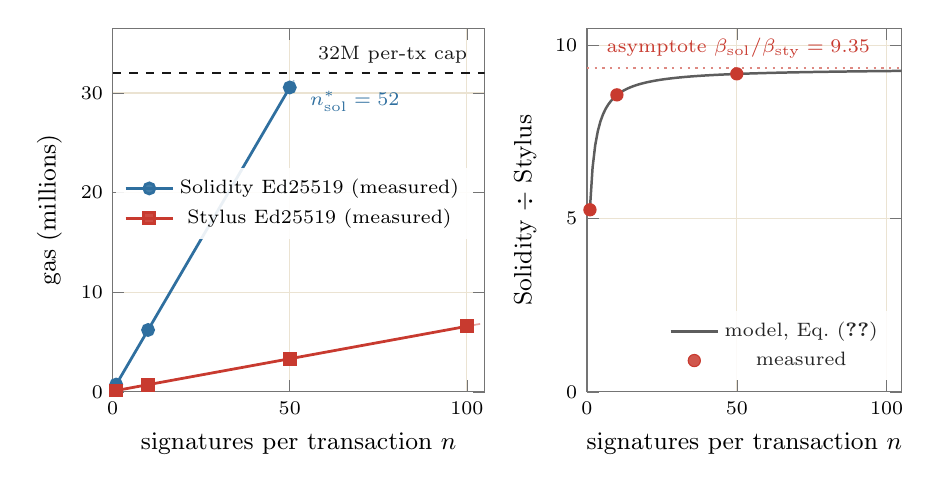
\begin{tikzpicture}
\begin{axis}[
  name=left, width=0.52\textwidth, height=6.2cm,
  xlabel={signatures per transaction $n$}, ylabel={gas (millions)},
  xmin=0, xmax=105, ymin=0, ymax=36.5,
  grid=major, grid style={washideep},
  axis line style={sumi!60}, tick style={sumi!60},
  legend style={font=\scriptsize,draw=none,fill=white,fill opacity=0.9,text opacity=1,at={(0.97,0.42)},anchor=south east},
  tick label style={font=\scriptsize}, label style={font=\small}]
  \addplot[shu!45,line width=0.6pt,dashed,domain=0:105,forget plot] {(74139+65088*x)/1e6};
  \addplot[ai!45,line width=0.6pt,dashed,domain=50:52.4,forget plot] {(128404+608542*x)/1e6};
  \addplot[ai,mark=*,mark size=2pt,line width=1pt] coordinates {(1,0.736502)(10,6.214368)(50,30.555405)};
  \addlegendentry{Solidity Ed25519 (measured)}
  \addplot[shu,mark=square*,mark size=2pt,line width=1pt] coordinates {(1,0.140063)(10,0.724659)(50,3.327511)(100,6.583441)};
  \addlegendentry{Stylus Ed25519 (measured)}
  \draw[sumi,dashed,line width=0.6pt] (axis cs:0,32) -- (axis cs:105,32) node[pos=0.98,above left,font=\scriptsize] {32M per-tx cap};
  \node[font=\scriptsize,ai,anchor=north west] at (axis cs:53,31.2) {$n^{*}_{\mathrm{sol}}=52$};
\end{axis}
\begin{axis}[
  at={(left.east)}, anchor=west, xshift=1.3cm,
  width=0.46\textwidth, height=6.2cm,
  xlabel={signatures per transaction $n$}, ylabel={Solidity $\div$ Stylus},
  xmin=0, xmax=105, ymin=0, ymax=10.5,
  grid=major, grid style={washideep},
  axis line style={sumi!60}, tick style={sumi!60},
  tick label style={font=\scriptsize}, label style={font=\small},
  legend style={font=\scriptsize,draw=none,fill=white,fill opacity=0.85,at={(0.97,0.03)},anchor=south east}]
  \addplot[sumi!70,line width=0.9pt,domain=1:105,samples=120] {(128404+608542*x)/(74139+65088*x)};
  \addlegendentry{model, Eq.~(\ref{eq:gas})}
  \addplot[only marks,mark=*,mark size=2.2pt,shu] coordinates {(1,5.258)(10,8.576)(50,9.183)};
  \addlegendentry{measured}
  \draw[shu!60,dotted,line width=0.8pt] (axis cs:0,9.35) -- (axis cs:105,9.35) node[pos=0.03,above right,font=\scriptsize,shu] {asymptote $\beta_{\mathrm{sol}}/\beta_{\mathrm{sty}}=9.35$};
\end{axis}
\end{tikzpicture}
\caption{Left: measured gas for strict Ed25519 verification with the linear fits of Eq.~(\ref{eq:gas}) dashed. Solidity crosses the 32M
per-transaction cap at 53 signatures; Stylus uses 21\% of it for 100. Right: the cost ratio rises toward the marginal-cost asymptote as fixed costs amortize.}
\label{fig:gas}
\end{figure}

For a single claim the difference is smaller but real. A full \ttt{submitClaim} cost 278{,}965 gas with the ECDSA
verifier and 372{,}294 with the Stylus Ed25519 verifier on chain, against 951{,}760 with the Solidity Ed25519 verifier on
a local EVM. ECDSA through the \ttt{ecrecover} precompile remains cheapest (about 5{,}000 gas per signature
marginal); Stylus earns its place precisely for schemes the EVM lacks.

% ================================================================ 7
\section{Why a Signature, and Why Not Yet a Hold Period}\label{sec:econ}

\subsection{Pixels cannot be the trust origin}
Figure~\ref{fig:forensics} reproduces the detection results of Wu et al.~\cite{wu2026forger}. The two forensic detectors retain
near-published performance on traditional splicing of the same documents and lose 0.27--0.36 AUC when the edit is made by
a current image model. No judge, human or machine, exceeds 0.60. An attester that reads pixels is therefore a
forgery-to-signature converter: every downstream check, however strong, faithfully certifies a fake. This is why tier-2
evidence is labelled as unestablished everywhere it appears, and why the merchant signature is the trust origin of tier 1.

\begin{figure}[!htb]
\centering
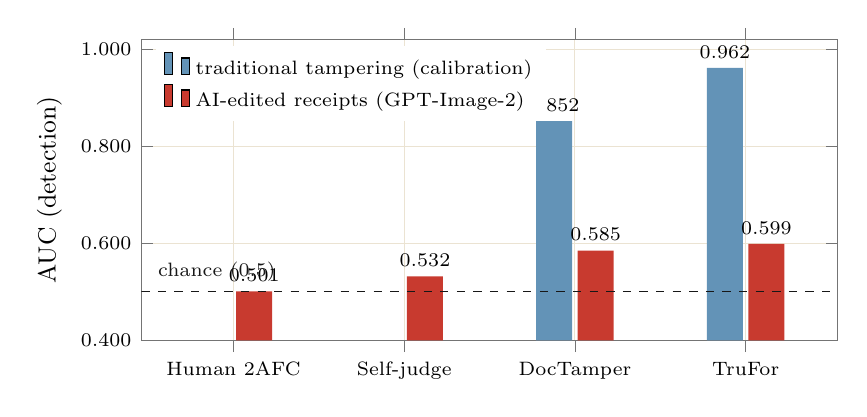
\begin{tikzpicture}
\begin{axis}[
  ybar, bar width=13pt, width=0.86\textwidth, height=5.4cm,
  ymin=0.4, ymax=1.02, ylabel={AUC (detection)},
  symbolic x coords={Human 2AFC,Self-judge,DocTamper,TruFor},
  xtick={Human 2AFC,Self-judge,DocTamper,TruFor}, enlarge x limits=0.18,
  /pgf/number format/fixed, /pgf/number format/precision=3, /pgf/number format/fixed zerofill,
  grid=major, grid style={washideep}, axis line style={sumi!60}, tick style={sumi!60},
  tick label style={font=\scriptsize}, label style={font=\small},
  nodes near coords, every node near coord/.append style={font=\scriptsize},
  nodes near coords align={vertical},
  legend style={font=\scriptsize,draw=none,at={(0.02,0.98)},anchor=north west},
  legend cell align=left]
  \addplot[fill=ai!75,draw=none] coordinates {(DocTamper,0.852)(TruFor,0.962)};
  \addlegendentry{traditional tampering (calibration)}
  \addplot[fill=shu,draw=none] coordinates {(Human 2AFC,0.501)(Self-judge,0.532)(DocTamper,0.585)(TruFor,0.599)};
  \addlegendentry{AI-edited receipts (GPT-Image-2)}
  \draw[sumi,dashed] (rel axis cs:0,0.163) -- (rel axis cs:1,0.163) node[pos=0.01,above right,font=\scriptsize] {chance (0.5)};
\end{axis}
\end{tikzpicture}
\caption{Forgery detection collapses on AI-edited receipts. Data from Wu et al.~\cite{wu2026forger} ($n=3{,}066$ forgeries; humans $N=120$, 365 pair votes).}
\label{fig:forensics}
\end{figure}

\subsection{Deterrence needs time}
Javarone, Leonardos and Ventre~\cite{javarone2026nft} model a farmer who creates $n$ linked identities and submits fraudulent claims for a
reward $R$ that vests after $T$ periods, while the issuer audits each claim per period with probability $a$ and detects fraud
with probability $s$. With $q_F$ the per-period eligibility persistence of a fraudulent claim, $k_F$ the cost per identity and $F$ a
forfeitable penalty, farming is deterred whenever
\begin{equation}\label{eq:deter}
q_F^{\,T} R \;\le\; k_F + T\,L(a)\,F,\qquad L(a) = -\ln(1-as),
\end{equation}
which gives the minimum audit rate for a vesting horizon $T$:
\begin{equation}\label{eq:amin}
a_{\min}(T) = \frac{1}{s}\left[1-\exp\!\left(-\frac{q_F^{\,T}R-k_F}{T\,F}\right)\right].
\end{equation}
At $T=0$ no audit rate deters: a claim that pays out immediately has no window in which to be checked. STOCKBACK settles in the
claim transaction, so $T=0$ today. Its defence is instead to raise $k_F$, the cost of a fraudulent claim, by requiring a merchant
signature, and to cap $R$ (Eq.~\ref{eq:reward}). Figure~\ref{fig:deter} plots Eq.~(\ref{eq:amin}) with the authors' own calibration to show what
a hold period would buy. It motivates the planned hold-and-void escrow in Section~\ref{sec:future}; it is not a measurement of STOCKBACK.

\begin{figure}[!htb]
\centering
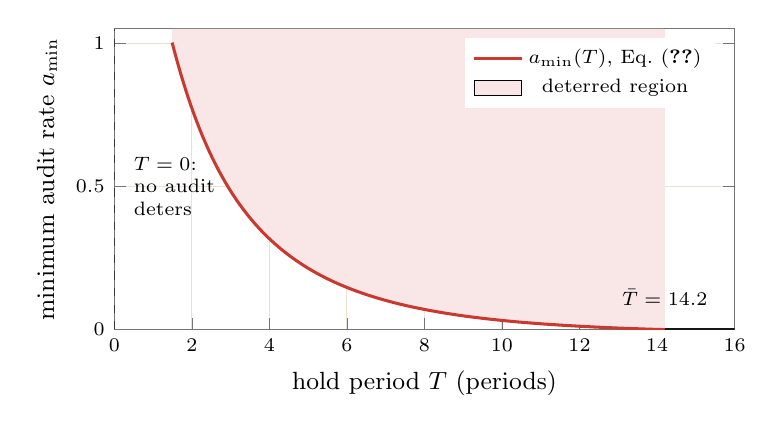
\begin{tikzpicture}
\begin{axis}[
  width=0.78\textwidth, height=5.4cm,
  xlabel={hold period $T$ (periods)}, ylabel={minimum audit rate $a_{\min}$},
  xmin=0, xmax=16, ymin=0, ymax=1.05,
  grid=major, grid style={washideep}, axis line style={sumi!60}, tick style={sumi!60},
  tick label style={font=\scriptsize}, label style={font=\small},
  legend style={font=\scriptsize,draw=none,at={(0.97,0.97)},anchor=north east}]
  \addplot[name path=f,shu,line width=1.1pt,domain=1.49:14.2,samples=160]
    {(1/0.6)*(1-exp(-((0.85^x)*100-10)/(x*50)))};
  \addlegendentry{$a_{\min}(T)$, Eq.~(\ref{eq:amin})}
  \addplot[name path=top,draw=none,domain=1.49:14.2,forget plot] {1.05};
  \addplot[shu!12,forget plot] fill between[of=f and top];
  \addlegendimage{area legend,fill=shu!12,draw=none}
  \addlegendentry{deterred region}
  \addplot[sumi,line width=1.1pt,domain=14.2:16,forget plot] {0};
  \draw[sumi,dashed] (axis cs:0,0) -- (axis cs:0,1.05);
  \node[font=\scriptsize,anchor=west,align=left] at (axis cs:0.25,0.5) {$T=0$:\\no audit\\deters};
  \node[font=\scriptsize,anchor=south] at (axis cs:14.2,0.05) {$\bar T=14.2$};
\end{axis}
\end{tikzpicture}
\caption{Deterrence frontier of Eq.~(\ref{eq:amin}) under the calibration of~\cite{javarone2026nft} ($R=100$, $k_F=10$, $q_F=0.85$, $s=0.6$, $F=50$). Longer holds need less auditing; with no hold, nothing deters.}
\label{fig:deter}
\end{figure}

\subsection{Replay is solved; Sybil resistance is not}
Proposition~\ref{prop:replay} prevents a receipt from counting twice. It does not tie a wallet to a person: Luo et al.\ found that
69.3\% of reported airdrop-hunter groups on Hop would have profited had they not been disqualified~\cite{luo2025airdrop}. STOCKBACK's
answer is structural rather than behavioural. Rewards attach to receipts, not identities, so a ``Sybil'' holding many
\emph{genuinely merchant-signed} receipts is simply a frequent customer. That argument holds only while the merchant key is not
compromised and, in this deployment, does not hold at all because the demo POS is public (Section~\ref{sec:limits}).

% ================================================================ 8
\section{Implementation and Evaluation}\label{sec:eval}

\paragraph{Code.} 791 lines of Solidity across eight contracts and their interfaces, 1{,}263 lines of Solidity tests,
251 lines of Rust, and about 4{,}600 lines of TypeScript for the web application, attester and simulated POS.

\paragraph{Tests.} Table~\ref{tab:tests} lists every suite and what it runs against. All results are from runs on 2 October 2026.

\begin{table}[!htb]
\centering\small
\caption{Test suites. ``Live'' suites run against the deployed contracts on Robinhood Chain testnet.}
\label{tab:tests}
\begin{tabularx}{\textwidth}{@{}l r >{\raggedright\arraybackslash}X l@{}}
\toprule
Suite & Count & Covers & Result\\
\midrule
Foundry (Solidity) & 83 & Unit, integration, security; 3 fuzz tests at 1{,}000 runs; 5 invariants at $128\times64$ calls (no replay, conservation, solvency, caps) & all pass\\
Rust (Stylus) & 5 & Strict Ed25519 on all 100 shared vectors; tampered digest, signature, length & all pass\\
Receipt signing (Node) & 20 & Valid receipt; tampering of each of 8 fields; wrong key; expiry; injection; fail-closed & all pass\\
Live integration & 22 & API rejections, \ttt{previewClaim}, a real \ttt{submitClaim}, duplicate rejection, keys missing & all pass\\
Browser (Chromium) & 11 & POS $\to$ QR link $\to$ verify $\to$ claim $\to$ replay rejected, real wallet & all pass\\
Secret scan & 1 & No secret value in 679 client build files or the git-tracked tree (negative control verified) & pass\\
\bottomrule
\end{tabularx}
\end{table}

\paragraph{On-chain activity.} As of 3 October 2026 the registry has settled \textbf{13 claims} from \textbf{3 wallets}
(11 Nike, 1 Apple, 1 Starbucks), allocating 248.19 demo units in total, and one sponsor budget has been funded in USDG. Representative transactions:

\begin{center}\small
\begin{tabular}{@{}lll@{}}
\toprule
Action & Transaction & Gas used\\
\midrule
Ed25519 attestation via Stylus (Apple, \inr 14{,}990) & \ttt{0x7fe2a51a\ldots d9c4} & 372{,}294\\
Merchant-signed receipt, browser (Nike, \inr 2{,}000) & \ttt{0xabd3b62b\ldots 5388} & 290{,}374\\
Merchant-signed receipt, API suite (Nike, \inr 2{,}000) & \ttt{0x801cac69\ldots 5627} & 288{,}025\\
Merchant-signed receipt, demo film (Nike, \inr 2{,}499) & \ttt{0x1fc40e3e\ldots a97} & 290{,}220\\
\midrule
USDG budget funding (100 USDG $\to$ 10{,}000 mNKE, mock USDG) & \ttt{0x3d8de149\ldots 6c6d} & 192{,}930\\
\bottomrule
\end{tabular}
\end{center}

The first Stylus claim cost more than later ones; we attribute the difference to first-write storage on that brand's
cap counters and vault, but we did not isolate it and report it as an observation, not a result.

% ================================================================ 9
\section{Findings from Building Against Deployed Code}\label{sec:findings}

Each finding below would have shipped as a silent defect had we trusted documentation or local tests alone.

\begin{enumerate}[leftmargin=*]
  \item \textbf{The upstream swap interface did not match the deployed router.} The forked code's \ttt{ISwapRouter} used
        the Uniswap V3 struct with a \ttt{deadline} field (selector \ttt{0x414bf389}). The router configured for Robinhood
        Chain mainnet does not contain that selector in its bytecode; it contains the SwapRouter02 selector \ttt{0x04e45aaf}.
        Every swap through it would have reverted. STOCKBACK's USDG adapter uses the SwapRouter02 layout, verified against
        bytecode.
  \item \textbf{A naive Solidity Ed25519 loop is quadratic.} Without rewinding the free-memory pointer between signatures,
        the library's allocations accumulate: 814M gas for 100 signatures against 60M with the rewind. Only the latter is a
        fair baseline, and it is the one we report.
  \item \textbf{Clipping a capped reward burns the receipt.} An early draft clipped rewards at the daily caps. Because the
        nullifier is burned on acceptance, a clipped claim would destroy the rest of the receipt's value; caps now reject (Eq.~\ref{eq:caps}).
  \item \textbf{Receipt identifiers collide across merchants.} Two merchants can issue the same invoice number. The attester
        namespaces the reference as \ttt{merchantId:receiptId} before salting, so each merchant has its own nullifier space.
  \item \textbf{An attestation must not outlive its receipt.} A one-hour claim deadline on a receipt that expires in ten
        minutes would extend the receipt's life on chain. The deadline is clamped to the receipt's expiry.
  \item \textbf{A second receipt link only changes the fragment.} Opening a new receipt link while already on the scan page
        changes only \ttt{location.hash}, so the page did not react. The browser suite caught it; the page now listens for
        \ttt{hashchange}.
  \item \textbf{In-memory rate limits are per instance.} Consecutive integration runs exhausted a per-IP limit of 20 requests per
        10 minutes and failed with 429s. The behaviour is correct, but on a serverless host each instance counts separately; it is
        listed as a limitation.
\end{enumerate}

% ================================================================ 10
\section{Trust Assumptions and Limitations}\label{sec:limits}

Stated plainly, in decreasing order of weight.
\begin{enumerate}[leftmargin=*]
  \item \textbf{The merchant is simulated, and its POS is public.} Anyone can mint a validly signed demo receipt. Tier 1 here
        demonstrates the mechanism, not fraud resistance; in production the key lives in the merchant's POS or HSM.
  \item \textbf{No hold period.} Rewards settle immediately, so refunded purchases keep their reward and no audit can claw anything
        back ($T=0$ in Eq.~\ref{eq:deter}).
  \item \textbf{Single attester key, single owner key.} Compromise is bounded by Proposition~\ref{prop:bound}, not prevented. There is no
        k-of-n attestation, timelock or multisig yet.
  \item \textbf{A receipt QR is a bearer token.} Whoever submits it first claims it. Copying an \emph{attestation} is useless, since the
        claimant is signed, but copying the \emph{receipt} before the customer claims is not prevented.
  \item \textbf{No proof of personhood.} Replay is prevented per receipt; Sybil resistance rests on the merchant key.
  \item \textbf{Mock assets.} Every brand asset and USDG on testnet is a labelled mock that refuses to deploy on production
        chains. Shares are not securities, and no brand partnership exists or is implied.
  \item \textbf{Amounts are public.} Merchant hash, amount and time are visible on chain; only identifiers are hidden.
  \item \textbf{Unaudited code.} The Solidity contracts and the Stylus verifier have not been externally audited.
\end{enumerate}

% ================================================================ 11
\section{Related Work}

\textbf{Document forensics.} GPT4o-Receipt~\cite{zhang2026receipt} found that LLM judges detect fully generated receipts mainly through arithmetic
errors; AIForge-Doc v2~\cite{wu2026forger} shows that localized AI edits defeat humans and detectors alike; FraudBench~\cite{yan2026fraudbench} extends
this to refund evidence. STOCKBACK does not try to detect forgeries; it removes the image from the trust path.
\textbf{Provable web data.} DECO~\cite{zhang2020deco} proves that data came from a TLS server without server cooperation, in about 5 seconds online
and 3--13 seconds of proving, and is the natural basis for tier 3. \textbf{Reward mechanism design.} Javarone et al.~\cite{javarone2026nft} characterize
deterrence under vesting and stochastic audit; Luo et al.~\cite{luo2025airdrop} measure hunter profits in airdrops; Yin and Wen~\cite{yin2026trust} model trust
arbitrage under generative AI. \textbf{Loyalty architecture.} Oamen et al.~\cite{oamen2025rewards} attribute coalition failure to the central operator and
propose brand-sovereign programs settled through trustless contracts and a universal asset; STOCKBACK's per-brand vaults and USDG
funding follow that architecture. \textbf{Primitives.} EIP-712~\cite{eip712}, ERC-4626~\cite{erc4626}, RFC~8032~\cite{rfc8032} and Arbitrum Stylus~\cite{stylus}.

% ================================================================ 12
\section{Future Work}\label{sec:future}
A hold-and-void escrow that releases shares after a per-brand return window and lets a merchant-signed refund void the claim,
making Eq.~(\ref{eq:deter}) satisfiable; a merchant key registry with rotation and revocation; k-of-n attestation verified as a
batch in Stylus, where Eq.~(\ref{eq:nmax}) leaves ample room; tier-3 evidence from zkTLS proofs of order and payment records;
amount privacy through range proofs; and, before any mainnet deployment, an external audit, a timelocked multisig owner and
issuer-authorized assets behind the existing jurisdiction adapter.

% ================================================================ 13
\section{Conclusion}
A reward is only as honest as the evidence it pays on, and a photograph is no longer evidence. STOCKBACK makes the trust origin a
signature, labels every claim with what was actually established, settles in one transaction whose checks are verified in Rust on
Arbitrum at up to $9.2\times$ less gas, and pays into vaults no one can administer. The design bounds what any single key can lose and
states what it does not yet do. Every number in this paper was measured on the deployed system or taken from the cited work.

\begin{center}\seal{0.32cm}\quad{\large\bfseries\color{sumi}Scan. Prove. Own.}\end{center}

% ================================================================ refs
\small
\begin{thebibliography}{99}\setlength{\itemsep}{1pt}
\bibitem{wu2026forger} J.~Wu, Y.~Zhou, D.~T.~Ng, X.~Shen, K.~Zewde, A.~Raj, T.~Duong, S.~Ren. \emph{When the Forger Is the Judge: GPT-Image-2 Cannot Recognize Its Own Faked Documents.} arXiv:2604.25213, 2026.
\bibitem{zhang2026receipt} Y.~Zhang, S.~Ren, et al. \emph{GPT4o-Receipt: A Dataset and Human Study for AI-Generated Document Forensics.} arXiv:2603.11442, 2026.
\bibitem{yan2026fraudbench} X.~Yan, B.~Chen, et al. \emph{FraudBench: A Multimodal Benchmark for Detecting AI-Generated Fraudulent Refund Evidence.} arXiv:2605.08820, 2026.
\bibitem{npci2026} National Payments Corporation of India. \emph{UPI Product Statistics}, September 2026. \url{https://www.npci.org.in/what-we-do/upi/product-statistics}.
\bibitem{yin2026trust} X.~Yin, F.~Wen. \emph{When Trust Attracts Fraud: AI and Trust Arbitrage.} Economics Letters; arXiv:2609.27404, 2026.
\bibitem{javarone2026nft} M.~A.~Javarone, S.~Leonardos, C.~Ventre. \emph{NFT-Based Reward Mechanisms: Sybil Farming, Vesting, and Stochastic Verification.} arXiv:2609.13064, 2026.
\bibitem{luo2025airdrop} J.~Luo, H.~Kang, S.~Zheng, X.~Liu. \emph{Toward Resilient Airdrop Mechanisms: Empirical Measurement of Hunter Profits and Airdrop Game Theory Modeling.} arXiv:2503.14316, 2025.
\bibitem{oamen2025rewards} P.~O.~Oamen, R.~Wesley, P.~Onobhayedo. \emph{Orchestrating Rewards in the Era of Intelligence-Driven Commerce.} arXiv:2512.00738, 2025 (citing the Bond Brand Loyalty Report 2020).
\bibitem{zhang2020deco} F.~Zhang, D.~Maram, H.~Malvai, S.~Goldfeder, A.~Juels. \emph{DECO: Liberating Web Data Using Decentralized Oracles for TLS.} ACM CCS 2020; arXiv:1909.00938.
\bibitem{eip712} R.~Bloemen, L.~Logvinov, J.~Evans. \emph{EIP-712: Typed Structured Data Hashing and Signing.} Ethereum Improvement Proposals, 2017.
\bibitem{erc4626} J.~Feng et al. \emph{ERC-4626: Tokenized Vaults.} Ethereum Improvement Proposals, 2021.
\bibitem{rfc8032} S.~Josefsson, I.~Liusvaara. \emph{Edwards-Curve Digital Signature Algorithm (EdDSA).} RFC 8032, IETF, 2017.
\bibitem{stylus} Offchain Labs. \emph{Arbitrum Stylus Documentation.} docs.arbitrum.io, 2026.
\bibitem{stockback} Project STOCKBACK. \emph{Source, tests, benchmarks and deployment records.} github.com/notwen123/STOCKBACK, 2026.
\end{thebibliography}

\vspace{6pt}
\noindent\rule{\textwidth}{0.4pt}
\footnotesize
\noindent STOCKBACK is hackathon software on a public testnet. Gas figures were measured on Robinhood Chain testnet (chain 46630) on
28 September 2026; reward parameters, claim counts and test results on 2 October 2026. Contract addresses are in
\ttt{deployments/46630.json}: registry \ttt{0x4273b12cD4A65c2180d4e65Bcb4254825cE64120}, Stylus verifier
\ttt{0x9ae8a390121ba71545e9923b333d60e7e3ccd3bd}. The merchant in the demo is simulated, all brand assets are mocks, and
no brand partnership exists or is implied. Figure~\ref{fig:forensics} and Figure~\ref{fig:deter} use data and parameters from the cited
papers, not STOCKBACK measurements. Nothing in this paper claims a result that was not measured.

\end{document}
